%%%%%%%%%%%%%%%%%%%%%%%%%%%%%%%%%%%%%%%%%
% baposter Portrait Poster
% LaTeX Template
% Version 1.0 (15/5/13)
%
% Created by:
% Brian Amberg (baposter@brian-amberg.de)
%
% This template has been downloaded from:
% http://www.LaTeXTemplates.com
%
% License:
% CC BY-NC-SA 3.0 (http://creativecommons.org/licenses/by-nc-sa/3.0/)
%
%%%%%%%%%%%%%%%%%%%%%%%%%%%%%%%%%%%%%%%%%

%----------------------------------------------------------------------------------------
%	PACKAGES AND OTHER DOCUMENT CONFIGURATIONS
%----------------------------------------------------------------------------------------

\documentclass[a1paper,portrait,fontscale=0.418]{baposter}

\usepackage[font=small,labelfont=bf]{caption} % Required for specifying captions to tables and figures
\usepackage{booktabs} % Horizontal rules in tables
\usepackage{relsize} % Used for making text smaller in some places
\usepackage{amsmath}
\usepackage{amsfonts}
\usepackage{amssymb}
\usepackage{amsthm}
\usepackage{algorithm2e}
\usepackage{listings}
\usepackage{xcolor}
\usepackage{tikz}
\usepackage{booktabs}
\usepackage{subfigure}
\usepackage[english]{babel}
\usepackage{blindtext}
\usepackage{pgfplots, pgfplotstable}
\usepackage{microtype}

\usepackage{tikz}
\usepackage{tikz-uml}
\tikzumlset{fill class=white}

\usepackage{graphicx}
\usepackage{adjustbox}
\usepackage{makecell}
\usetikzlibrary{arrows}


\lstdefinelanguage{JavaScript}{
  keywords={typeof, new, true, false, catch, function, return, null, catch, switch, var, if, in, while, do, else, case, break},
  keywordstyle=\color{blue}\bfseries,
  ndkeywords={class, export, boolean, throw, implements, import, this},
  ndkeywordstyle=\color{darkgray}\bfseries,
  identifierstyle=\color{black},
  sensitive=false,
  comment=[l]{//},
  morecomment=[s]{/*}{*/},
  commentstyle=\color{purple}\ttfamily,
  stringstyle=\color{red}\ttfamily,
  morestring=[b]',
  morestring=[b]"
}
\lstset{
   language=JavaScript,
   %backgroundcolor=\color{lightgray},
   extendedchars=true,
   basicstyle=\footnotesize\ttfamily,
   showstringspaces=false,
   showspaces=false,
   numbers=left,
   numberstyle=\footnotesize,
   numbersep=9pt,
   tabsize=2,
   breaklines=true,
   showtabs=false,
   captionpos=b
}

\newcommand{\js}[1]{\lstinline[language=Javascript]$#1$}


\graphicspath{{figures/}} % Directory in which figures are stored

\definecolor{bordercol}{RGB}{40,40,40} % Border color of content boxes
\definecolor{headercol1}{RGB}{240,240,240} % Background color for the header in the content boxes (left side)
\definecolor{headercol2}{RGB}{80,80,80} % Background color for the header in the content boxes (right side)
\definecolor{headerfontcol}{RGB}{0,0,0} % Text color for the header text in the content boxes
\definecolor{boxcolor}{RGB}{255,255,255} % Background color for the content in the content boxes


\begin{document}

\background{ % Set the background to an image (background.pdf)
\begin{tikzpicture}[remember picture,overlay]
\draw (current page.north west)+(-2em,2em) node[anchor=north west]
{
\includegraphics[height=1.1\textheight]{background.pdf}};
\end{tikzpicture}
}

\begin{poster}{
grid=false,
borderColor=bordercol, % Border color of content boxes
headerColorOne=headercol1, % Background color for the header in the content boxes (left side)
headerColorTwo=headercol2, % Background color for the header in the content boxes (right side)
headerFontColor=headerfontcol, % Text color for the header text in the content boxes
boxColorOne=boxcolor, % Background color for the content in the content boxes
headershape=roundedright, % Specify the rounded corner in the content box headers
headerfont=\Large\sf\bf, % Font modifiers for the text in the content box headers
textborder=rectangle,
background=user,
headerborder=open, % Change to closed for a line under the content box headers
boxshade=plain
}
{}
%
%----------------------------------------------------------------------------------------
%	TITLE AND AUTHOR NAME
%----------------------------------------------------------------------------------------
%
{\sf\bf Sherlock: A Profiling Tool to Find Opportunities for Early Property Initialization} % Poster title
{\vspace{1em}Tarek Auel, David G\"usewell\\ % Author names
{\smaller tarek.auel@gmail.com, d.guesewell@web.de}} % Author email addresses
{
\includegraphics[]{logo}} % University/lab logo

%----------------------------------------------------------------------------------------
%	INTRODUCTION
%----------------------------------------------------------------------------------------

\begin{posterbox}[name=introduction,column=0,row=0]{Introduction}
With Sherlock, we introduce a new profiling tool to find opportunities for \textbf{early object property and array element initialization} as shown in Listing \ref{list1}. In order to do this, the analysis has to keep track of the usage of the elements or properties. The \textbf{expected benefits} for such early property initializations are (i) \textbf{improved code readability}, and (ii) \textbf{improved performance} because the computation time spent in \textbf{push} and \textbf{reverse} calls is now saved.

\begin{center}
\begin{tabular}{|c}
\begin{lstlisting}[language=Javascript]
var a = [1, 2, 3]
a.push(4);
b = a.reverse();
/*
optimization: var a = [4, 3, 2, 1]
              b = a;
*/

\end{lstlisting}

\end{tabular}
\captionof{lstlisting}{Example for early property initialization}
\label{list1}
\end{center}

The main goals of Sherlock are to find these opportunities for early property initialization and keep the number of false positives as low as possible at the same time. Due to this, in some use cases Sherlock prefers not to optimizing a value instead of running in a potential false positive situation.
\end{posterbox}
%----------------------------------------------------------------------------------------
%	METHODS
%----------------------------------------------------------------------------------------

\begin{posterbox}[name=methods,column=0,below=introduction]{Overview}
Overall \textbf{Sherlock is an implemented plugin for Jalangi}. Jalangi is a dynamic framework for JavaScript. By transforming the code and adding hooks, it allows the user to monitor almost every operation performed by the execution. Sherlock implements the callbacks which called by Jalangi in order to perform the desired dynamic analysis. Before the code is analyzed by Sherlock it is instrumented using Esprima, Estraverse and Escodegen in order to be able to track events that are not exposed by Jalangi such as the end of a branch. This additions allows to safely optimize coding which could not have optimized otherwise.

\begin{center}
\adjustbox{width=6cm}{
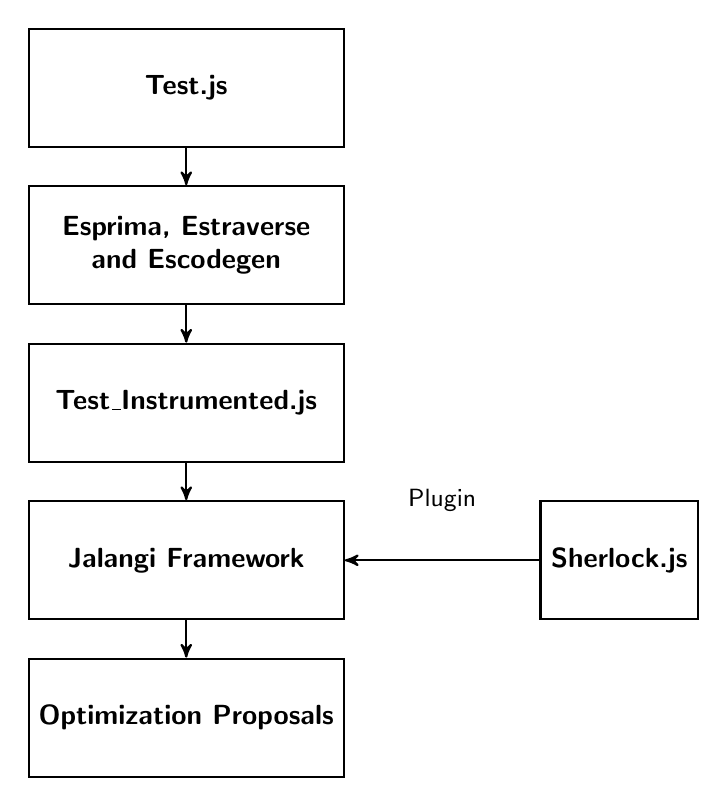
\begin{tikzpicture}[->,>=stealth',shorten >=0pt,auto,node distance=2cm,
  thick,main node/.style={rectangle,draw,font=\sffamily\bfseries}, hidden node/.style={},
  minimum width=4cm, minimum height=1.5cm]
	\node[main node] (A) []{Test.js};
	\node[main node] (B) [below of=A]{\makecell{Esprima, Estraverse\\and Escodegen}};
	\node[main node] (C) [below of=B]{Test\_Instrumented.js};
	\node[main node] (D) [below of=C]{Jalangi Framework};			
	\node[main node, node distance=5.5cm, minimum width = 2cm] (E) [right of=D]{Sherlock.js};			
	\node[main node] (F) [below of=D]{Optimization Proposals};					
	
	  \path[->,every node/.style={font=\sffamily\small}]
	  (A) edge node[] {} (B)
	  (B) edge node[] {} (C)
	  (C) edge node[] {} (D)
	  (E) edge node[above] {Plugin} (D)
	  (D) edge node[] {} (F)	  	  	  	  	  
	  ;
\end{tikzpicture}
}
\captionof{figure}{Optimization process using Sherlock with Jalangi}
\label{fig1}  
\end{center}
%
%To track every object or array created during one execution, Sherlock uses a data structure called \textit{Reference}. One \textit{Reference} object may keep track of multiple references to one object/array. Furthermore Sherlock maintains some variables during the execution.
%
%\begin{itemize}
%\item{\textbf{callStack}} is an array of \js{strings} that represent the current call stack. The call stack is cleared, if \js{endExpression} is called. 
%
%\item{\textbf{allRefs}} is an array of \js{References} that the plugin tracks at the moment.
%\end{itemize}
%
%Whenever an object property or an array element is read, it cannot be optimized further. 
%In order to do this, Sherlock can lock array elements or object properties if they have been read.
\end{posterbox}

%----------------------------------------------------------------------------------------
%	REFERENCES
%----------------------------------------------------------------------------------------

\begin{posterbox}[name=references,column=0,below=methods]{References}

\smaller % Reduce the font size in this block
\renewcommand{\section}[2]{\vskip 0.05em} % Get rid of the default "References" section title
\nocite{*} % Insert publications even if they are not cited in the poster

\bibliographystyle{unsrt}
\bibliography{sample} % Use sample.bib as the bibliography file
\end{posterbox}



%----------------------------------------------------------------------------------------
%	RESULTS 
%----------------------------------------------------------------------------------------

\begin{posterbox}[name=results1,span=2,column=1,row=0]{Sherlock} 
Sherlock is constantly evaluated with a set of self written test-cases. The tests proves which potential optimizations Sherlock can identify. But nevertheless, Sherlock may skip potential optimizations if it either may not be safe to optimize the code or Sherlock does not recognize that it is possible, yet.\\

\textbf{Supported early property optimizations} \\ 
The following listing shows two examples for coding that Sherlocks optimizes.

\begin{center}
\begin{tabular}{|c c |c }
\begin{lstlisting}[language=Javascript]
var a = []; 
a[0] = 1;
//optimization: var a = [1];
var b = {}; 
b.a = 5;
//optimization: var b = {a: 5};
\end{lstlisting}
& &
\begin{lstlisting}[language=Javascript]
var a =[1,2,3,4];  
a.reverse();
// optimization: var a = [4,3,2,1];
\end{lstlisting} 
\end{tabular}
\setlength{\tabcolsep}{12em}
\captionof{lstlisting}{Examples for typical potential early property and array
element initialization}
\end{center}

The left example of Listing 2 shows a typical potential of early property and array element initialization which is covered by Sherlock. But Sherlock does not only optimize elements or properties that are set later, but also many builtin standard JavaScript functions. For the right example, Sherlock recognizes that the array could be initialized in reverse order.
%In order to decide which built functions it can optimize, Sherlock divide the functions in four different groups.
%
%
%\begin{itemize}
%\item{\textbf{Ignore}}
%\item{\textbf{Lock reference}}
%\item{\textbf{Call on unlocked}}
%\item{\textbf{Other}}
%\end{itemize}


In the left example of Listing 3 the only supported optimization would be made for \textit{a}. \textit{b} must not be optimized, because this would change the semantics (in particular the output of line $6$). \textit{c}  and \textit{d} show two corner cases that are not supported, because Sherlock cannot distinguish using Jalangi if the \textit{length} was used as index or as part of the assignment.\\
Conditioned initialization should only be done, if the optimization is always true. In the conditioned example only \textit{b} can be optimized, because it is independent of the branching in line $2$. \textit{a} depends on \textit{cond} and must not be optimized

\begin{center}
\begin{tabular}{|l l |l }
\begin{lstlisting}[language=Javascript]
var a = [];
a[a.length] = 0;
a[1] = 1;
//optimization: var a =[0,1];
var b = [1, 2, 3];
console.log(b.length);
b[3] = 4;
//cannot be optimized
var c = [];
c[c.length - 1] = 0;
//cannot be optimized
var d = [];
d[0] = d.length - 1;
//cannot be optimized
\end{lstlisting}
& &
\begin{lstlisting}[language=Javascript]
var a = []
if (cond) {
  a[0] = 1;
  var b = []
  b[0] = 1;
	//optimization: var b =[1];
}
\end{lstlisting} 
\end{tabular}
\setlength{\tabcolsep}{12em}
\captionof{lstlisting}{Examples for coding that can be optimized by Sherlock}
\end{center}

\textbf{Evaluation} \\ 
Sherlock still misses some potential optimizations. So far Sherlock cannot deal with objects that are created by constructors, because this introduces many situations where Sherlock has to keep track of even more properties of the coding and where often Sherlock has to discard a optimization because it may change the logic, because of side effects or other reasons.

The following figure shows the runtime difference of optimized and unoptimized array initializations. Even though Sherlock can inspect the Octane benchmarking suite, it does not find any optimization. The reason for that is the capabilities of Sherlock are still limited and that the benchmarks do not use plain objects or arrays. Especially they do not add elements within the same scope and they do not use builtin JavaScript functions that Sherlock can optimize.


 
\begin{center}
\begin{tikzpicture}
        \pgfplotsset{
            scale only axis
            }
    \begin{axis}[    	   
	   %ymin = 0,
	   %ymax = 50,
	   %xmin = 0,
	   %xmax = 100,
	   width=12cm,
             height=5cm,
	   xlabel=Array Size,
            axis x line=bottom,
            axis y line=left,
%            enlarge x limits=0.1,
            grid = major,
            grid style={dashed, gray!30},
            ylabel=Runtime in ms,
            legend style={at={(0.1,-0.1)}, anchor=north},
            bar shift=-7,
            legend cell align=left,
            legend entries={
                Unoptimized,
                Optimized},
	       legend pos= north west
         ]        
        \addplot[color = black, dotted, ultra thick] table  {data1.txt};
        \addplot[color = black, dashed, ultra thick] table  {data2.txt};        
        
                        
    \end{axis}
    \end{tikzpicture}

\end{center}

\end{posterbox}

%----------------------------------------------------------------------------------------
%	Conclusion
%----------------------------------------------------------------------------------------

\begin{posterbox}[name=conclusion,span=2,column=1,below=results1]{Conclusion} 
We introduced a new profiling tool to find opportunities for early property initialization, named Sherlock. While there is still a long way to go to find all possible early property optimizations our results show that Sherlock is able to find a broad range of them.

%
%Nunc sit amet sem ut nulla tincidunt mattis vel nec mauris. Vestibulum odio tellus, lobortis. Vel adipiscing, Aliquam dictum, ligula egestas commodo posuere, lectus lectus congue ligula, sed posuere urna lectus at nisi. Aenean commodo risus ut dolor (viverra scelerisque). Nullam varius, lacus et interdum hendrerit, odio orci ultrices mauris, id interdum eros mauris at urna. Fusce in nisi eros, sit amet volutpat turpis, \textbf{porttior magna} (commodo blandit euismod) \textbf{facilisis ornate magnis} (dis magnis). 
%
%%------------------------------------------------
%
%\begin{center}
%
\includegraphics[width=0.49\linewidth]{placeholder}
%
\includegraphics[width=0.49\linewidth]{placeholder}
%\captionof{figure}{Figure caption 1 (left); Figure caption 2 (right)}
%\end{center}
%
%%------------------------------------------------
%
%Aliquam ac justo lectus. Nunc ultrices aliquet purus non dictum. Nulla facilisi. Quisque vitae urna non purus sollicitudin venenatis. Aliquam erat volutpat. Cum sociis natoque penatibus et magnis dis parturient montes, nascetur ridiculus mus. In hendrerit tortor sed massa consequat eu viverra justo porta. Ut nec felis sem, non elementum.
%
%%------------------------------------------------
%
%\begin{center}
%
\includegraphics[width=0.8\linewidth]{placeholder}
%\captionof{figure}{Figure caption}
%\end{center}
%
%%------------------------------------------------
%
%Nunc sit amet sem ut nulla tincidunt mattis vel nec mauris. Vestibulum odio tellus, lobortis. Vel adipiscing, Aliquam dictum, ligula egestas commodo posuere, lectus lectus congue ligula, sed posuere urna lectus at nisi. Aenean commodo risus ut dolor (viverra scelerisque). Nullam varius, lacus et interdum hendrerit, odio orci ultrices mauris, id interdum eros mauris at urna. Fusce in nisi eros, sit amet volutpat turpis, \textbf{porttior magna} (commodo blandit euismod) \textbf{facilisis ornate magnis} (dis magnis). Aliquam ac justo lectus. Nunc ultrices aliquet purus non dictum. Nulla facilisi. Quisque vitae urna non purus sollicitudin venenatis. Aliquam erat volutpat. Cum sociis natoque penatibus et magnis dis parturient montes, nascetur ridiculus mus. In hendrerit tortor sed massa consequat eu viverra justo porta. Ut nec felis sem, non elementum.
\end{posterbox}

%----------------------------------------------------------------------------------------
%	ACKNOWLEDGEMENTS
%----------------------------------------------------------------------------------------

%\begin{posterbox}[name=acknowledgements,span=2,column=1,below=conclusion]{Acknowledgements}

%\smaller % Reduce the font size in this block
%Fusce mattis tellus ac odio imperdiet lobortis. Cum sociis natoque penatibus et magnis dis parturient montes, nascetur ridiculus mus. Phasellus commodo blandit euismod. Ut porttitor cursus magna.
%\end{posterbox}


%----------------------------------------------------------------------------------------

\end{poster}

\end{document}